\documentclass[12pt,a4paper]{article}

% Packages
\usepackage{amsmath}
\usepackage{amsfonts}
\usepackage{amssymb}
\usepackage{graphicx}
\usepackage[margin=1in]{geometry}
\usepackage{enumitem}
\usepackage[hidelinks]{hyperref}
\usepackage{xcolor}

% Title
\title{Homework Report for Computer Vision}
\author{Yu Xiang, Luo}
\date{\today}

\begin{document}

\maketitle

\[
	\href{https://github.com/YuXiangLo/Computer-Vision}{\text{\textcolor{blue}{You can check this github for more information}}}
\]

\begin{enumerate}[label=(\alph*)]
	\item Dilation\\
		\\
		\fbox{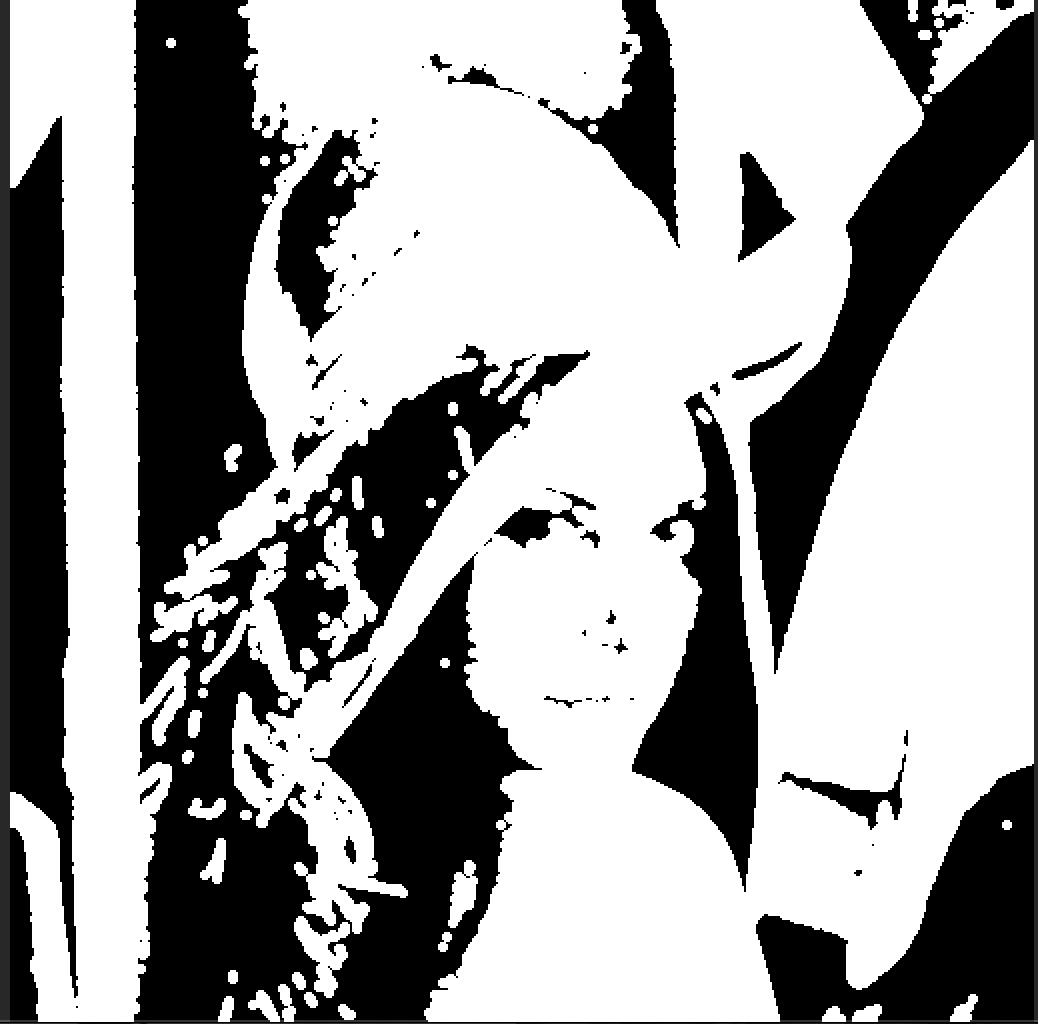
\includegraphics[width=0.4\textwidth]{img/dilation.png}}\\
		\\
		\fbox{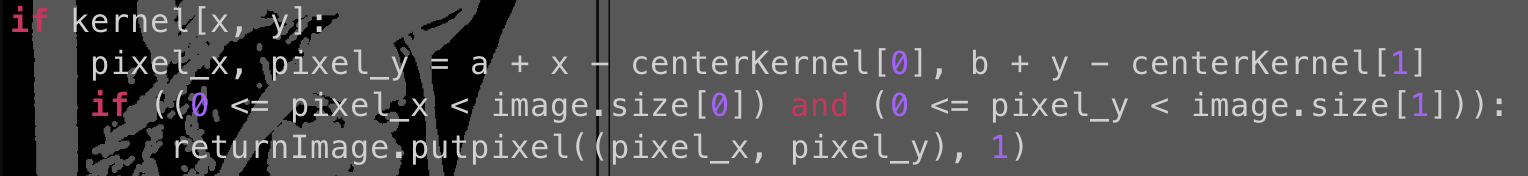
\includegraphics[width=0.9\textwidth]{img/dilation_code.png}}
		\\ \\  
		In this code, \texttt{a, b} means the current coordinate, and we put the pixel to $1$ if there's any point is $1$ in its kernel space.\\
		\newpage
	\item Erosion\\
		\fbox{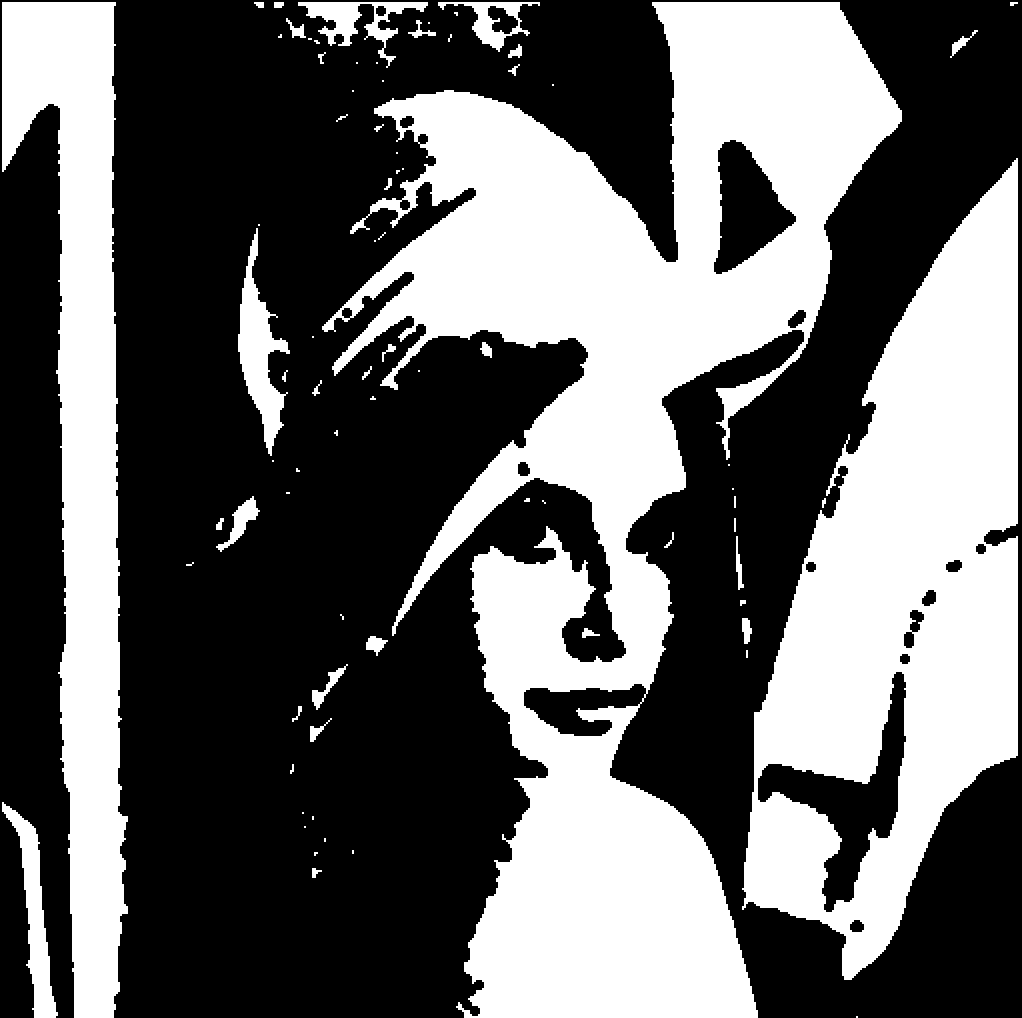
\includegraphics[width=0.4\textwidth]{img/erosion.png}}\\
		\fbox{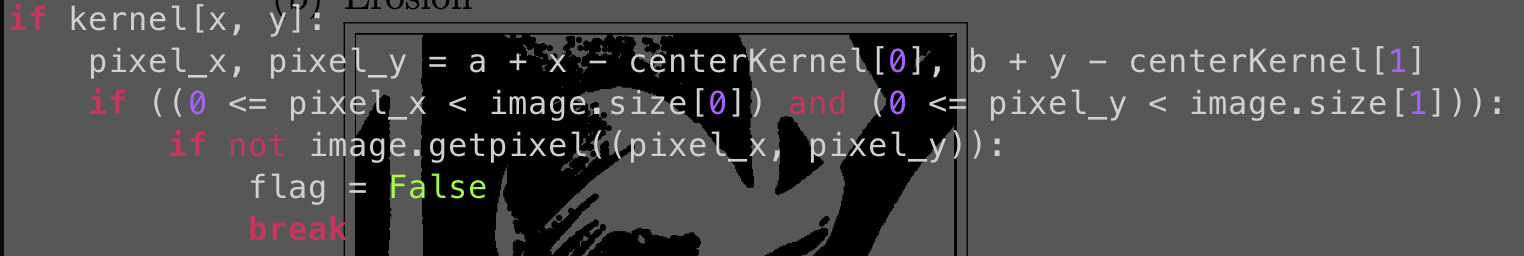
\includegraphics[width=0.9\textwidth]{img/erosion_code.png}}\\
		In this code, flag is true only if all the pixel in kernel space are 1. If \texttt{flag} is \texttt{True}, the pixel of \texttt{(a, b)} would set to $1$.
		\newpage
	\item Opening\\
		\fbox{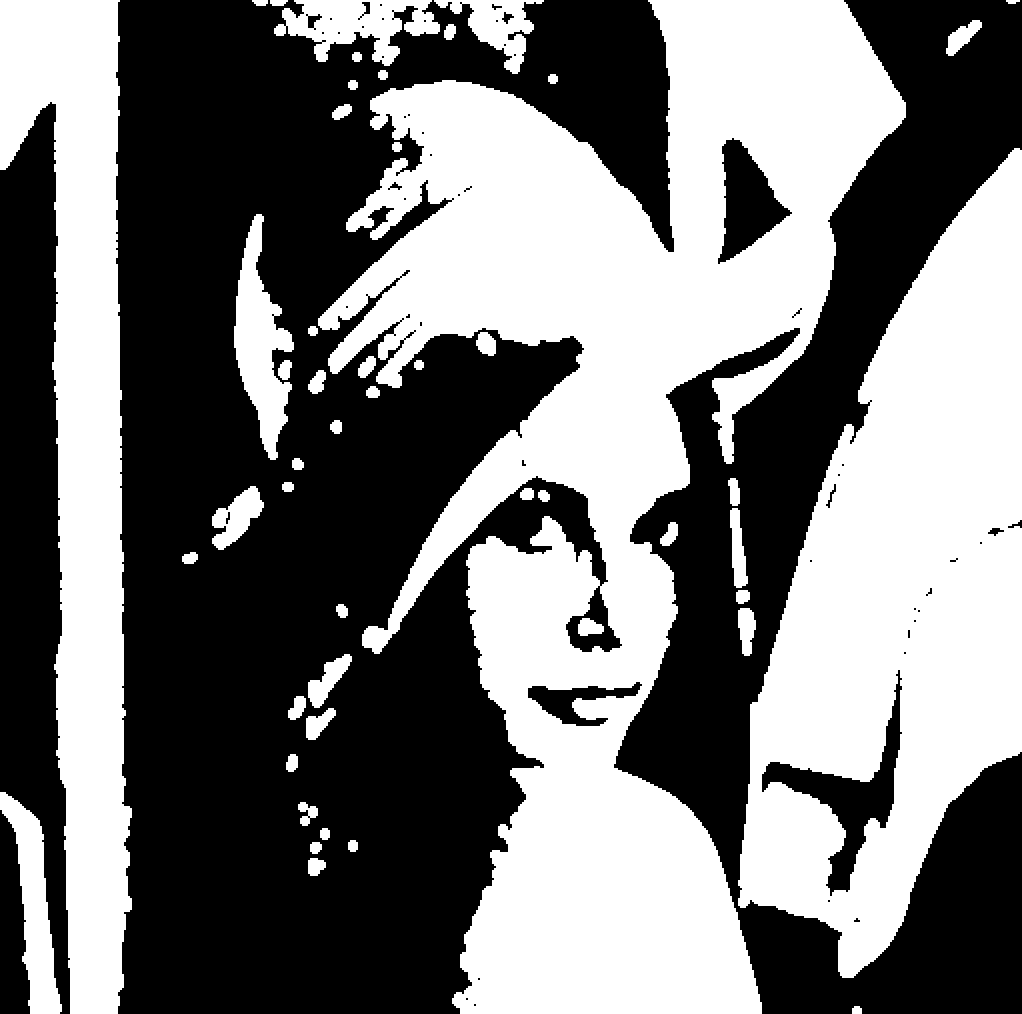
\includegraphics[width=0.4\textwidth]{img/opening.png}}
	\item Closing\\
		\fbox{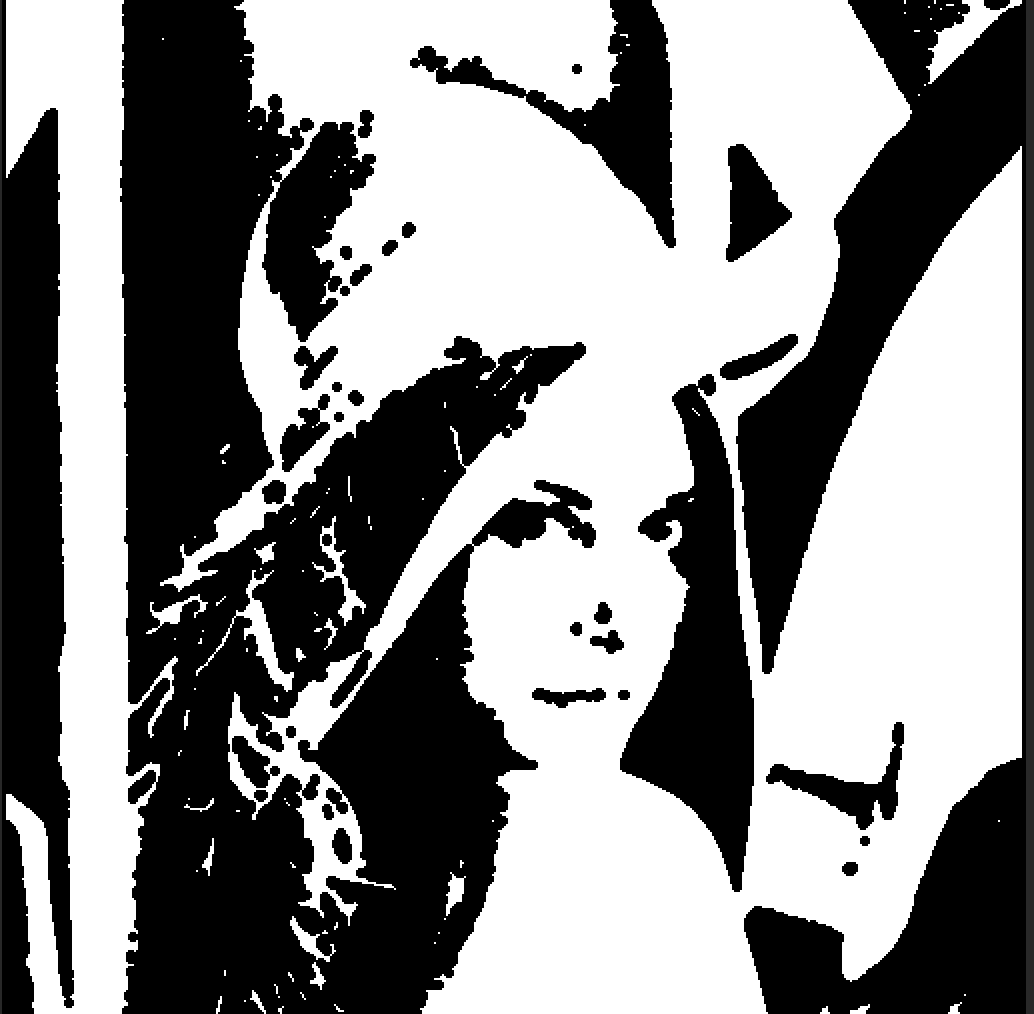
\includegraphics[width=0.4\textwidth]{img/closing.png}}\\
		\fbox{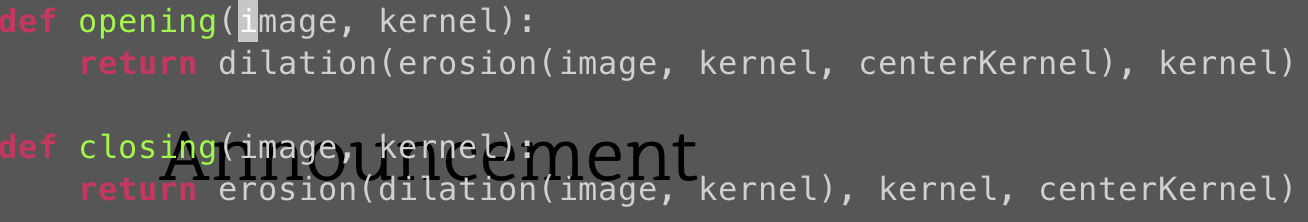
\includegraphics[width=0.9\textwidth]{img/open_close_code.png}}\\
		Opening and closing are simply the combinated usage of dilation and erosion.
		\newpage
	\item Hit-and-miss\\
		\fbox{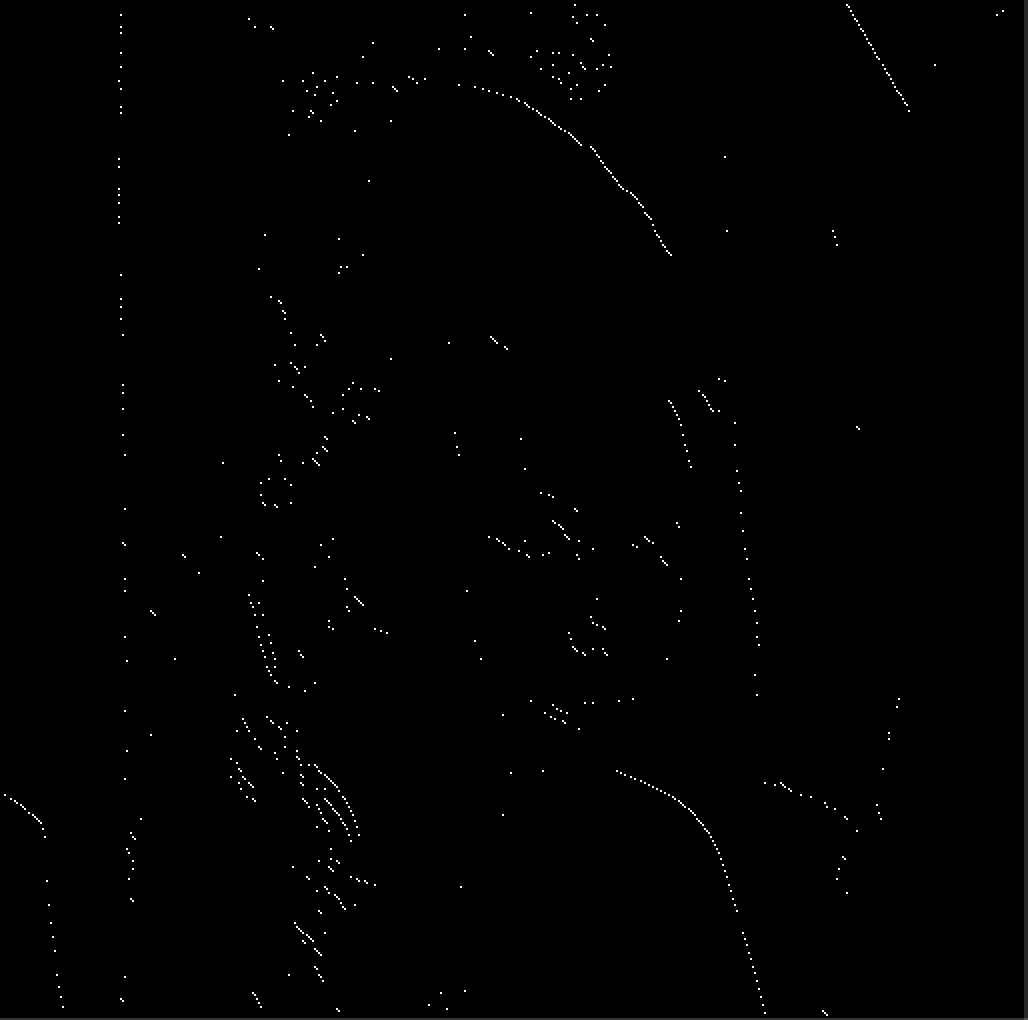
\includegraphics[width=0.4\textwidth]{img/hit_and_miss.png}}\\
		\fbox{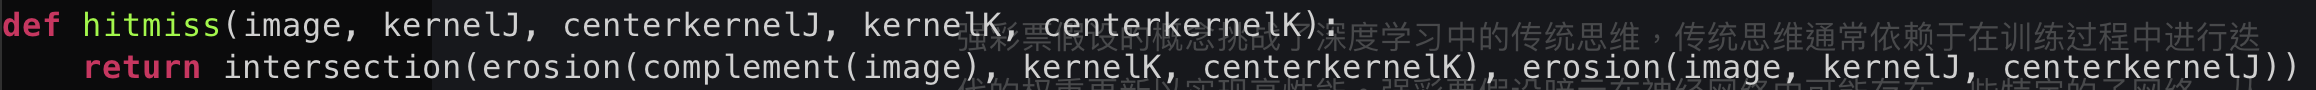
\includegraphics[width=0.9\textwidth]{img/ham_code.png}}\\
		Details of intersection and complement can be found at the source code.
		

\end{enumerate}



\end{document}
